% This file was created by matlab2tikz.
%
%The latest updates can be retrieved from
%  http://www.mathworks.com/matlabcentral/fileexchange/22022-matlab2tikz-matlab2tikz
%where you can also make suggestions and rate matlab2tikz.
%
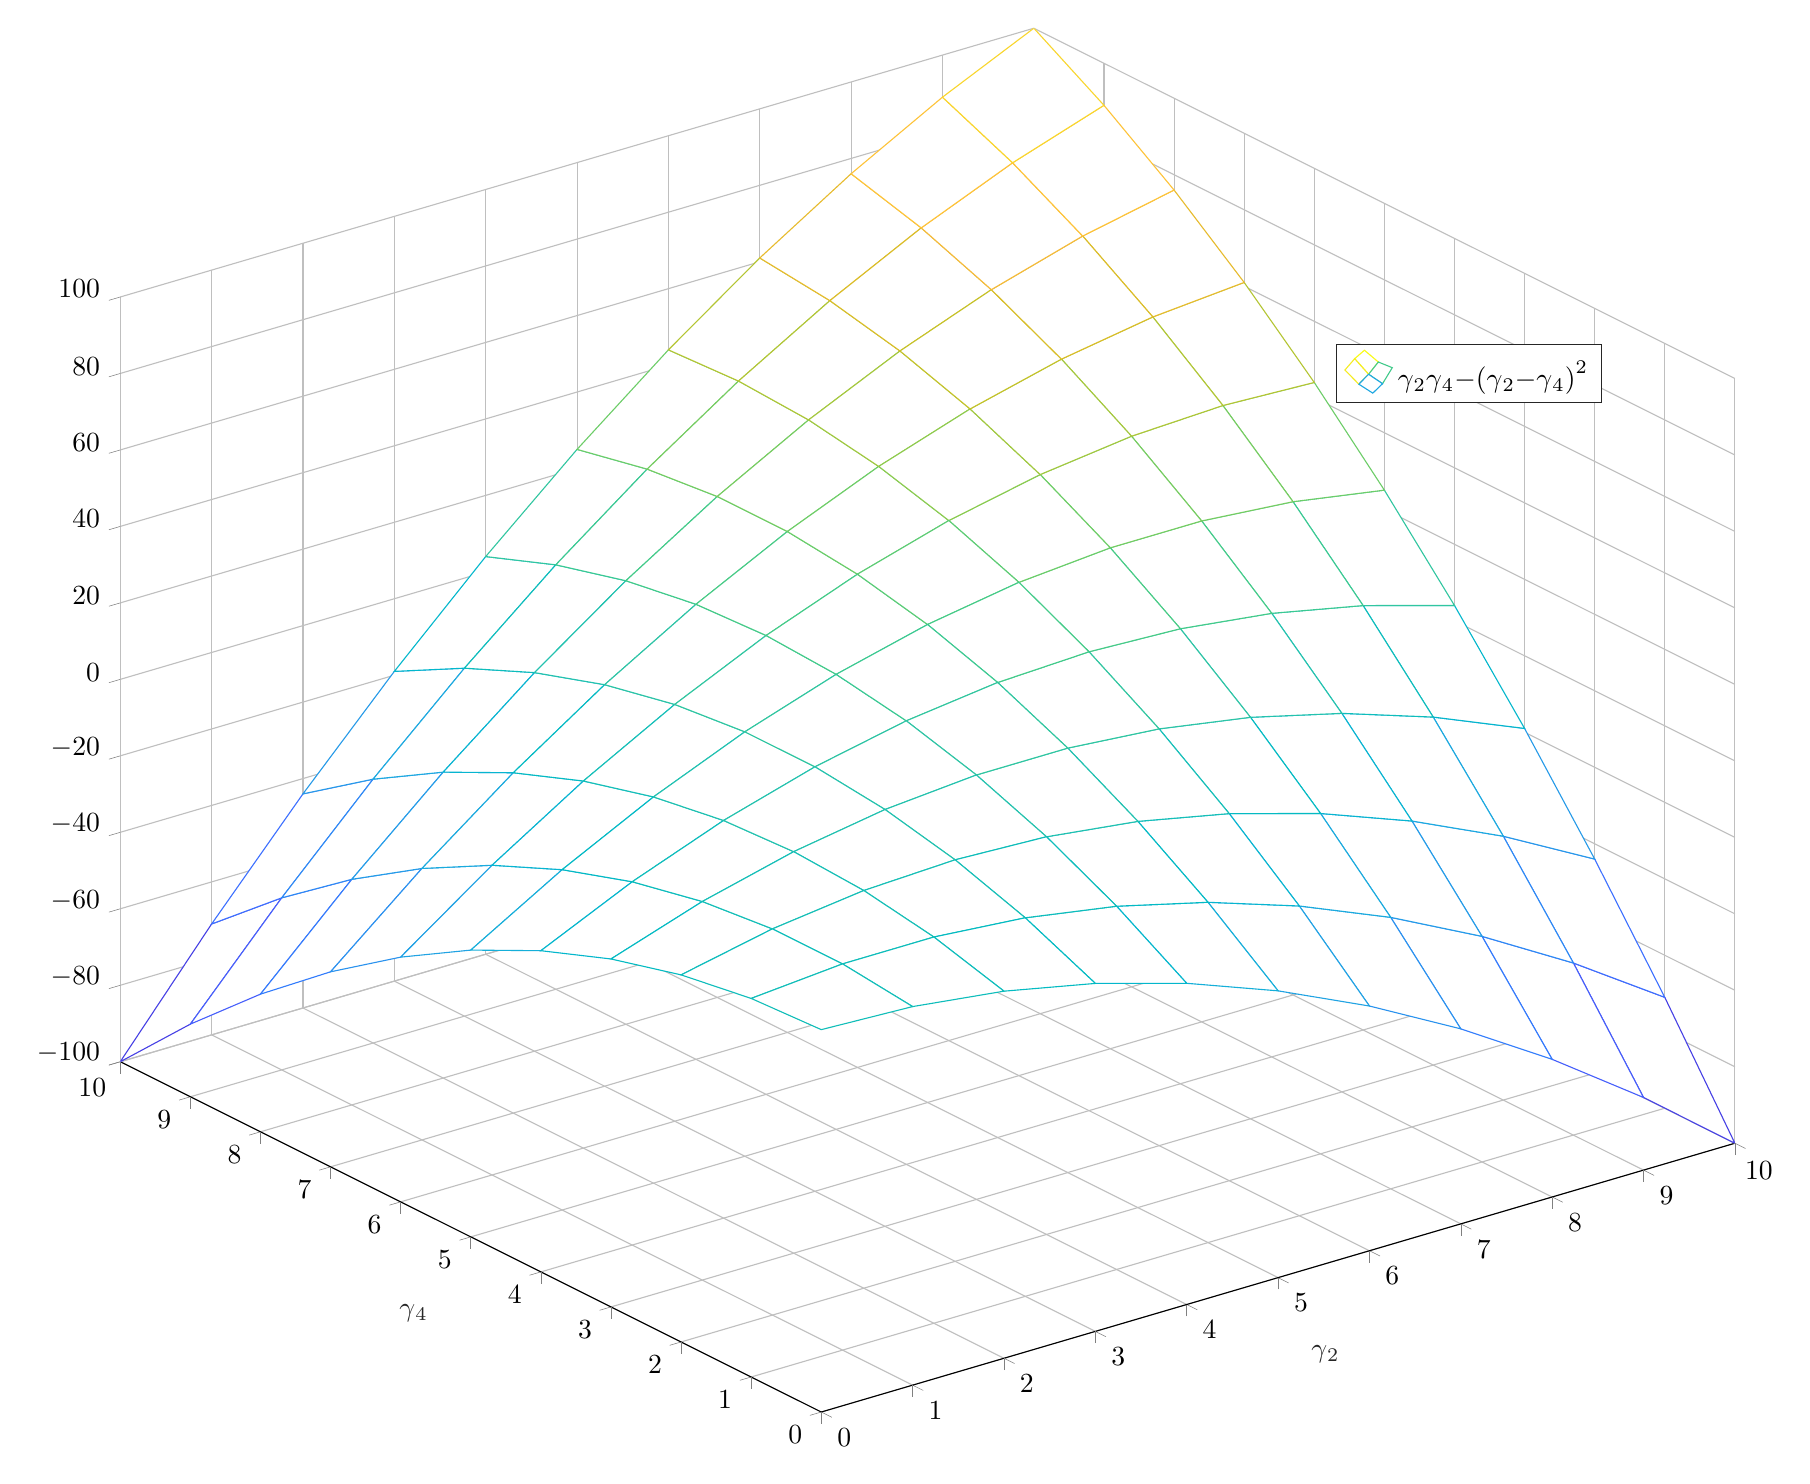
\begin{tikzpicture}

\begin{axis}[%
width=8.073in,
height=6.919in,
at={(1.354in,0.934in)},
scale only axis,
xmin=0,
xmax=10,
tick align=outside,
xlabel style={font=\color{white!15!black}},
xlabel={$\gamma{}_\text{2}$},
ymin=0,
ymax=10,
ylabel style={font=\color{white!15!black}},
ylabel={$\gamma{}_\text{4}$},
zmin=-100,
zmax=100,
view={-37.5}{30},
axis background/.style={fill=white},
axis x line*=bottom,
axis y line*=left,
axis z line*=left,
xmajorgrids,
ymajorgrids,
zmajorgrids,
legend style={at={(0.753,0.729)}, anchor=south west, legend cell align=left, align=left, draw=white!15!black}
]

\addplot3[%
surf,
shader=flat corner, fill=white, z buffer=sort, colormap={mymap}{[1pt] rgb(0pt)=(0.2422,0.1504,0.6603); rgb(1pt)=(0.25039,0.164995,0.707614); rgb(2pt)=(0.257771,0.181781,0.751138); rgb(3pt)=(0.264729,0.197757,0.795214); rgb(4pt)=(0.270648,0.214676,0.836371); rgb(5pt)=(0.275114,0.234238,0.870986); rgb(6pt)=(0.2783,0.255871,0.899071); rgb(7pt)=(0.280333,0.278233,0.9221); rgb(8pt)=(0.281338,0.300595,0.941376); rgb(9pt)=(0.281014,0.322757,0.957886); rgb(10pt)=(0.279467,0.344671,0.971676); rgb(11pt)=(0.275971,0.366681,0.982905); rgb(12pt)=(0.269914,0.3892,0.9906); rgb(13pt)=(0.260243,0.412329,0.995157); rgb(14pt)=(0.244033,0.435833,0.998833); rgb(15pt)=(0.220643,0.460257,0.997286); rgb(16pt)=(0.196333,0.484719,0.989152); rgb(17pt)=(0.183405,0.507371,0.979795); rgb(18pt)=(0.178643,0.528857,0.968157); rgb(19pt)=(0.176438,0.549905,0.952019); rgb(20pt)=(0.168743,0.570262,0.935871); rgb(21pt)=(0.154,0.5902,0.9218); rgb(22pt)=(0.146029,0.609119,0.907857); rgb(23pt)=(0.138024,0.627629,0.89729); rgb(24pt)=(0.124814,0.645929,0.888343); rgb(25pt)=(0.111252,0.6635,0.876314); rgb(26pt)=(0.0952095,0.679829,0.859781); rgb(27pt)=(0.0688714,0.694771,0.839357); rgb(28pt)=(0.0296667,0.708167,0.816333); rgb(29pt)=(0.00357143,0.720267,0.7917); rgb(30pt)=(0.00665714,0.731214,0.766014); rgb(31pt)=(0.0433286,0.741095,0.73941); rgb(32pt)=(0.0963952,0.75,0.712038); rgb(33pt)=(0.140771,0.7584,0.684157); rgb(34pt)=(0.1717,0.766962,0.655443); rgb(35pt)=(0.193767,0.775767,0.6251); rgb(36pt)=(0.216086,0.7843,0.5923); rgb(37pt)=(0.246957,0.791795,0.556743); rgb(38pt)=(0.290614,0.79729,0.518829); rgb(39pt)=(0.340643,0.8008,0.478857); rgb(40pt)=(0.3909,0.802871,0.435448); rgb(41pt)=(0.445629,0.802419,0.390919); rgb(42pt)=(0.5044,0.7993,0.348); rgb(43pt)=(0.561562,0.794233,0.304481); rgb(44pt)=(0.617395,0.787619,0.261238); rgb(45pt)=(0.671986,0.779271,0.2227); rgb(46pt)=(0.7242,0.769843,0.191029); rgb(47pt)=(0.773833,0.759805,0.16461); rgb(48pt)=(0.820314,0.749814,0.153529); rgb(49pt)=(0.863433,0.7406,0.159633); rgb(50pt)=(0.903543,0.733029,0.177414); rgb(51pt)=(0.939257,0.728786,0.209957); rgb(52pt)=(0.972757,0.729771,0.239443); rgb(53pt)=(0.995648,0.743371,0.237148); rgb(54pt)=(0.996986,0.765857,0.219943); rgb(55pt)=(0.995205,0.789252,0.202762); rgb(56pt)=(0.9892,0.813567,0.188533); rgb(57pt)=(0.978629,0.838629,0.176557); rgb(58pt)=(0.967648,0.8639,0.16429); rgb(59pt)=(0.96101,0.889019,0.153676); rgb(60pt)=(0.959671,0.913457,0.142257); rgb(61pt)=(0.962795,0.937338,0.12651); rgb(62pt)=(0.969114,0.960629,0.106362); rgb(63pt)=(0.9769,0.9839,0.0805)}, mesh/rows=11]
table[row sep=crcr, point meta=\thisrow{c}] {%
%
x	y	z	c\\
0	0	0	0\\
0	1	-1	-1\\
0	2	-4	-4\\
0	3	-9	-9\\
0	4	-16	-16\\
0	5	-25	-25\\
0	6	-36	-36\\
0	7	-49	-49\\
0	8	-64	-64\\
0	9	-81	-81\\
0	10	-100	-100\\
1	0	-1	-1\\
1	1	1	1\\
1	2	1	1\\
1	3	-1	-1\\
1	4	-5	-5\\
1	5	-11	-11\\
1	6	-19	-19\\
1	7	-29	-29\\
1	8	-41	-41\\
1	9	-55	-55\\
1	10	-71	-71\\
2	0	-4	-4\\
2	1	1	1\\
2	2	4	4\\
2	3	5	5\\
2	4	4	4\\
2	5	1	1\\
2	6	-4	-4\\
2	7	-11	-11\\
2	8	-20	-20\\
2	9	-31	-31\\
2	10	-44	-44\\
3	0	-9	-9\\
3	1	-1	-1\\
3	2	5	5\\
3	3	9	9\\
3	4	11	11\\
3	5	11	11\\
3	6	9	9\\
3	7	5	5\\
3	8	-1	-1\\
3	9	-9	-9\\
3	10	-19	-19\\
4	0	-16	-16\\
4	1	-5	-5\\
4	2	4	4\\
4	3	11	11\\
4	4	16	16\\
4	5	19	19\\
4	6	20	20\\
4	7	19	19\\
4	8	16	16\\
4	9	11	11\\
4	10	4	4\\
5	0	-25	-25\\
5	1	-11	-11\\
5	2	1	1\\
5	3	11	11\\
5	4	19	19\\
5	5	25	25\\
5	6	29	29\\
5	7	31	31\\
5	8	31	31\\
5	9	29	29\\
5	10	25	25\\
6	0	-36	-36\\
6	1	-19	-19\\
6	2	-4	-4\\
6	3	9	9\\
6	4	20	20\\
6	5	29	29\\
6	6	36	36\\
6	7	41	41\\
6	8	44	44\\
6	9	45	45\\
6	10	44	44\\
7	0	-49	-49\\
7	1	-29	-29\\
7	2	-11	-11\\
7	3	5	5\\
7	4	19	19\\
7	5	31	31\\
7	6	41	41\\
7	7	49	49\\
7	8	55	55\\
7	9	59	59\\
7	10	61	61\\
8	0	-64	-64\\
8	1	-41	-41\\
8	2	-20	-20\\
8	3	-1	-1\\
8	4	16	16\\
8	5	31	31\\
8	6	44	44\\
8	7	55	55\\
8	8	64	64\\
8	9	71	71\\
8	10	76	76\\
9	0	-81	-81\\
9	1	-55	-55\\
9	2	-31	-31\\
9	3	-9	-9\\
9	4	11	11\\
9	5	29	29\\
9	6	45	45\\
9	7	59	59\\
9	8	71	71\\
9	9	81	81\\
9	10	89	89\\
10	0	-100	-100\\
10	1	-71	-71\\
10	2	-44	-44\\
10	3	-19	-19\\
10	4	4	4\\
10	5	25	25\\
10	6	44	44\\
10	7	61	61\\
10	8	76	76\\
10	9	89	89\\
10	10	100	100\\
};
\addlegendentry{$\gamma{}_\text{2}\gamma{}_\text{4}\text{ - (}\gamma{}_\text{2}\text{ - }\gamma{}_\text{4}\text{)}^\text{2}$}

\end{axis}
\end{tikzpicture}%